\section{The Takamaka Language for Smart Contracts}\label{sec:takamaka}

This section gives a short introduction to the Takamaka subset of
Java that we use for writing smart contracts in this paper.
This language has been introduced in~\cite{Spoto19}. A full tutorial
is available online, as part of the documentation of the Hotmoka
blockchain that runs smart contracts written
in Takamaka~\cite{hotmoka_repository}. This section introduces only
the essential notions that are needed to understand the subsequent sections.

\begin{figure}[t]
  \begin{center}
    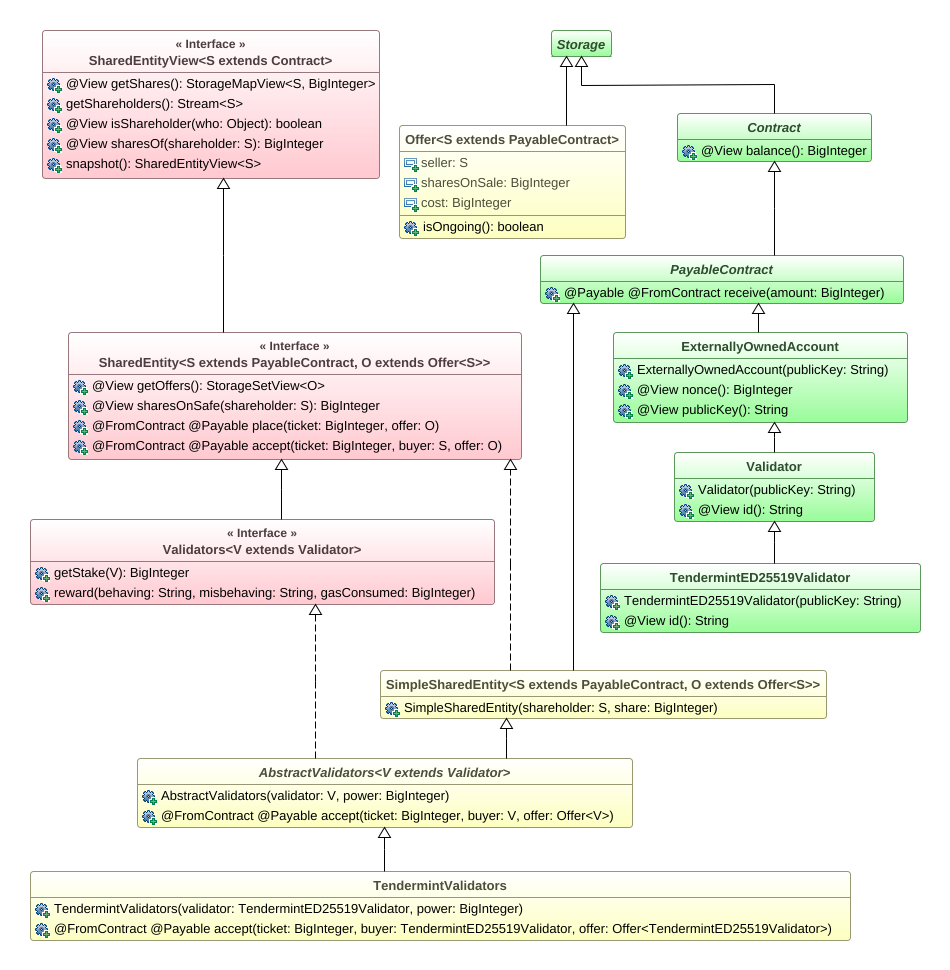
\includegraphics[width=12.2cm]{entities-hierarchy.png}
  \end{center}
  \caption{The hierarchy of Takamaka classes that implement accounts, shared entities and validators. Their source code can be found inside the Java project \textsf{\url{https://github.com/Hotmoka/hotmoka/tree/master/io-takamaka-code}}.}\label{fig:hierarchy-entities}
\end{figure}

